% !TeX program = xelatex
\documentclass[aspectratio=169,11pt]{beamer}

\usepackage[vietnamese]{babel}
% Biên dịch bằng XeLaTeX để dùng trực tiếp glyph Unicode tiếng Việt,
% tránh việc pdfLaTeX thay Roboto bằng font T5/VNR.
\usepackage{fontspec}
\setsansfont{Roboto}[
  UprightFont=*-Regular,
  BoldFont=*-Bold,
  ItalicFont=*-Italic,
  BoldItalicFont=*-BoldItalic]
\setmainfont{Roboto}[
  UprightFont=*-Regular,
  BoldFont=*-Bold,
  ItalicFont=*-Italic,
  BoldItalicFont=*-BoldItalic]
% Dùng cùng Roboto cho các đoạn \texttt để tránh trộn font trong sơ đồ.
\setmonofont{Roboto}[
  UprightFont=*-Regular,
  BoldFont=*-Bold]
\usepackage{booktabs}
\usepackage{array}
\usepackage{tabularx}
\usepackage{graphicx}
\usepackage{tikz}
\usepackage{amsmath}
\usepackage{fontawesome5}
\usepackage{ragged2e}
\usetikzlibrary{arrows.meta,positioning,calc,shapes.geometric,fit,backgrounds}

\definecolor{Navy}{HTML}{12355B}
\definecolor{Blue}{HTML}{1D70B8}
\definecolor{Sky}{HTML}{EAF4FF}
\definecolor{Cyan}{HTML}{3AA6B9}
\definecolor{Orange}{HTML}{F4A261}
\definecolor{Green}{HTML}{2A9D8F}
\definecolor{Red}{HTML}{D65A5A}
\definecolor{Ink}{HTML}{1F2937}
\definecolor{Gray}{HTML}{6B7280}
\definecolor{LightGray}{HTML}{F4F6F8}
\definecolor{Line}{HTML}{D8DEE9}

\colorlet{xface}{Blue}
\colorlet{xfaceDark}{Navy}
\colorlet{xfaceLight}{Sky}
\colorlet{xfaceGreen}{Green}
\colorlet{xfaceOrange}{Orange}

\usetheme{default}
\setbeamertemplate{navigation symbols}{}
\setbeamertemplate{frametitle continuation}{}
\setbeamersize{text margin left=0.65cm,text margin right=0.65cm}
\setbeamercolor{normal text}{fg=Ink,bg=white}
\setbeamercolor{structure}{fg=Blue}
\setbeamercolor{frametitle}{fg=Ink,bg=white}
\setbeamerfont{frametitle}{series=\bfseries,size=\Large}
\setbeamercolor{block title}{fg=white,bg=Blue}
\setbeamercolor{block body}{fg=Ink,bg=Sky}
\setbeamertemplate{blocks}[rounded][shadow=false]
\setbeamertemplate{frametitle}{%
  \vspace{0.18cm}
  \begin{beamercolorbox}[wd=\paperwidth,ht=0.58cm,dp=0.12cm,leftskip=0.65cm,rightskip=0.65cm]{frametitle}
    \insertframetitle
  \end{beamercolorbox}
  \vspace{-0.18cm}
  \hspace{0.65cm}\textcolor{Line}{\rule{0.91\paperwidth}{0.6pt}}
}
\setbeamertemplate{footline}{%
  \leavevmode%
  \hbox{%
    \begin{beamercolorbox}[wd=.72\paperwidth,ht=0.34cm,dp=0.11cm,leftskip=0.65cm]{author in head/foot}%
      \scriptsize\textcolor{Gray}{xFace --- Edge AI trên Luckfox RV1106}
    \end{beamercolorbox}%
    \begin{beamercolorbox}[wd=.28\paperwidth,ht=0.34cm,dp=0.11cm,rightskip=0.65cm plus1fil]{date in head/foot}%
      \scriptsize\textcolor{Gray}{\insertframenumber/\inserttotalframenumber}
    \end{beamercolorbox}}}
\setbeamertemplate{itemize item}{\textcolor{Blue}{\scriptsize\faCircle}}
\setbeamertemplate{itemize subitem}{\textcolor{Orange}{\tiny\faAngleRight}}
\setlength{\parskip}{3pt}

\newcommand{\metric}[2]{%
  \begin{beamercolorbox}[wd=0.22\textwidth,rounded=true,center,sep=0.8ex]{block body}
    {\color{xface}\Large\bfseries #1}\\[-0.2ex]
    {\scriptsize #2}
  \end{beamercolorbox}}

\title{\textbf{xFace}}
\subtitle{Hệ thống Edge AI phát hiện, nhận diện và điểm danh khuôn mặt\\trên Luckfox RV1106}
\author{Võ Quốc Kha \and Trần Ngọc Tú \and Huỳnh Đăng Khoa}
\institute{Học phần Công nghệ số nâng cao}
\date{Tháng 8 năm 2026}

\begin{document}

% Slide 1
{
\setbeamertemplate{footline}{}
\begin{frame}[plain]
  \begin{tikzpicture}[remember picture,overlay]
    \fill[Navy] (current page.south west) rectangle (current page.north east);
    \fill[Blue!75] (current page.south west) -- ($(current page.south west)+(5.8,0)$)
      -- ($(current page.north west)+(9.8,0)$) -- (current page.north west) -- cycle;
    \draw[white,opacity=.16,line width=.8pt] ($(current page.south east)+(-3.0,2.2)$) circle (1.8);
    \draw[white,opacity=.12,line width=.8pt] ($(current page.north east)+(-2.6,-1.6)$) circle (1.1);
    \foreach \x/\y in {11.2/6.1,12.0/5.5,13.1/6.7,14.2/5.9,10.7/3.5,13.8/2.7,12.4/1.6}
      {\fill[Orange,opacity=.65] (\x,\y) circle (.045);}
    \node[anchor=west,text width=11.5cm] at ($(current page.west)+(0.9,0.55)$) {
      {\color{Orange}\large\bfseries BÁO CÁO HỌC PHẦN CÔNG NGHỆ SỐ NÂNG CAO}\\[0.25cm]
      {\color{white}\fontsize{29}{33}\selectfont\bfseries xFace}\\[0.15cm]
      {\color{white!88}\Large Hệ thống Edge AI phát hiện, nhận diện và điểm danh khuôn mặt trên Luckfox RV1106}\\[0.65cm]
      {\color{white}\normalsize Võ Quốc Kha \quad Trần Ngọc Tú \quad Huỳnh Đăng Khoa}\\[0.1cm]
      {\color{white!72}\small Tháng 8 năm 2026}
    };
    \node[anchor=south east] at ($(current page.south east)+(-.75,.55)$)
      {\color{white!75}\faCamera\quad\faMicrochip\quad\faChartLine\quad\faGraduationCap};
  \end{tikzpicture}
\end{frame}
}

% Slide 2
\begin{frame}{1. Bài toán và mục tiêu}
\begin{columns}[T,onlytextwidth]
  \column{0.48\textwidth}
  \begin{block}{Bài toán}
  \begin{itemize}
    \item Điểm danh khuôn mặt thường phụ thuộc máy chủ hoặc Internet.
    \item Thiết bị nhúng bị giới hạn về bộ nhớ và năng lực tính toán.
    \item Hệ thống cần hoạt động tại chỗ và bảo vệ dữ liệu sinh trắc học.
  \end{itemize}
  \end{block}
  \column{0.48\textwidth}
  \begin{block}{Mục tiêu của xFace}
  \begin{itemize}
    \item Train detector khuôn mặt từ dữ liệu thực tế.
    \item Chuyển đổi YOLOv5s sang RKNN INT8 cho RV1106.
    \item Tích hợp nhận diện, phân biệt thật--giả, RTSP và web local.
  \end{itemize}
  \end{block}
\end{columns}
\vspace{0.8em}
\centering
\color{xfaceDark}\large Camera $\rightarrow$ AI trên thiết bị $\rightarrow$ Điểm danh trong mạng nội bộ
\end{frame}

% Slide 3
\begin{frame}{2. Bộ dữ liệu Roboflow}
\begin{columns}[T,onlytextwidth]
  \column{0.55\textwidth}
  \centering
  \begin{tabular}{lrr}
    \toprule
    \textbf{Tập} & \textbf{Ảnh gốc} & \textbf{Bản xuất} \\
    \midrule
    Training & 2.829 & 8.487 \\
    Validation & 354 & 354 \\
    Test & 353 & 353 \\
    \midrule
    \textbf{Tổng} & \textbf{3.536} & \textbf{9.194} \\
    \bottomrule
  \end{tabular}
  \vspace{0.8em}

  \small Một lớp: Face Detection; giấy phép CC BY 4.0.
  \column{0.41\textwidth}
  \begin{block}{Tiền xử lý và data augmentation}
  \begin{itemize}
    \item Auto-Orient, ảnh 640$\times$640.
    \item Lật ngang.
    \item Brightness $[-15\%,+15\%]$.
    \item Exposure $[-10\%,+10\%]$.
    \item Blur tối đa 1,5 pixel.
  \end{itemize}
  \end{block}
\end{columns}
\end{frame}

% Slide 4
\begin{frame}{3. Training YOLOv5s}
\begin{columns}[T,onlytextwidth]
  \column{0.69\textwidth}
    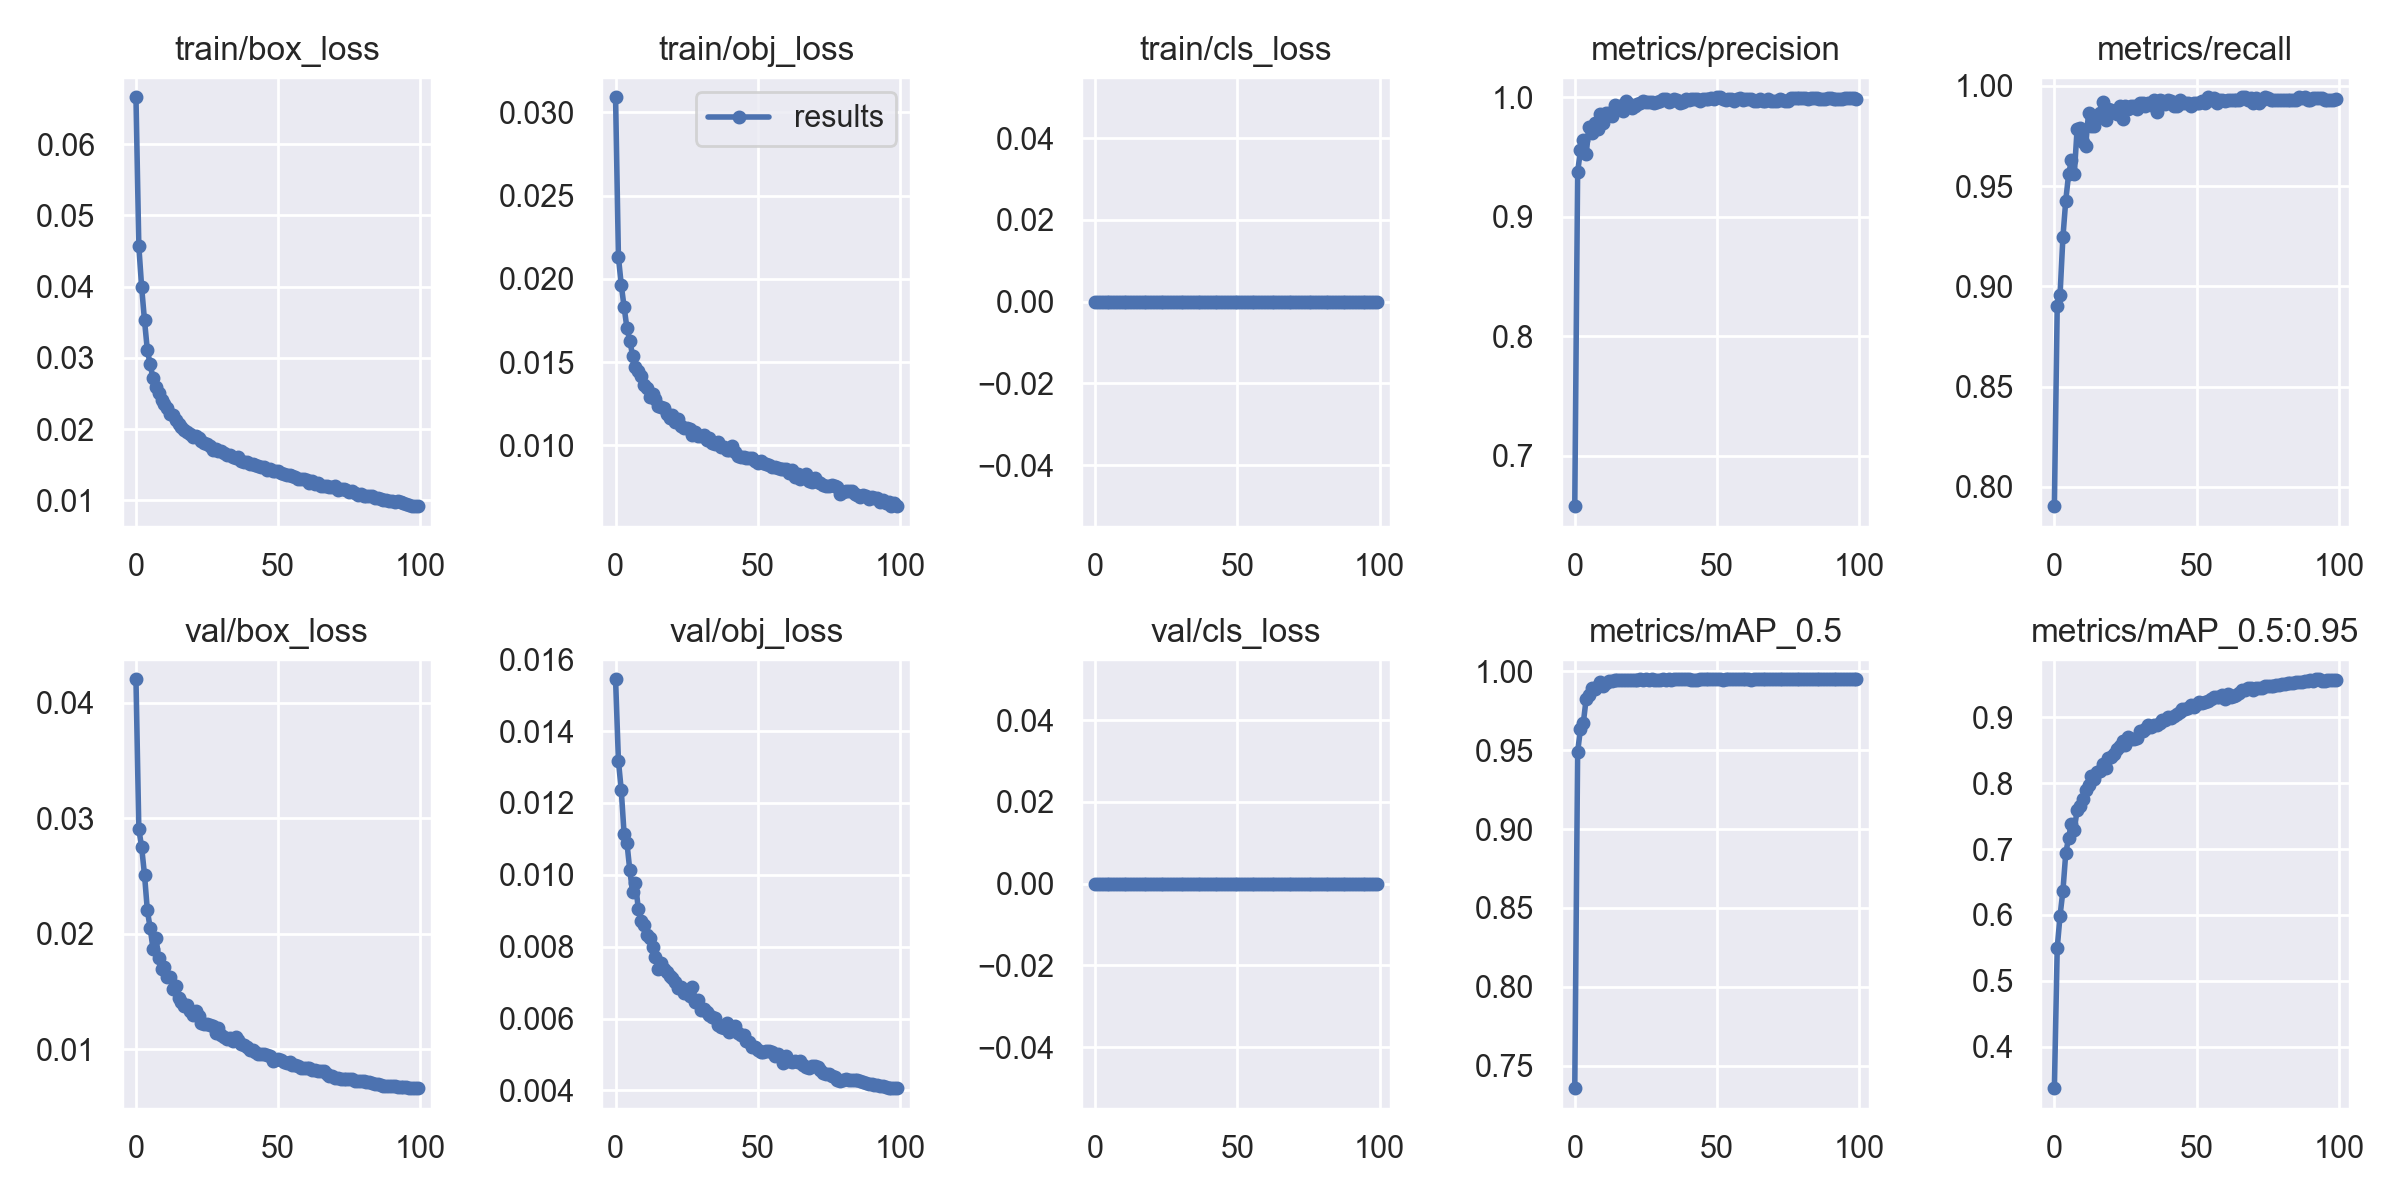
\includegraphics[width=\linewidth]{paper_assets/yolov5_training_results.png}
  \column{0.28\textwidth}
  \begin{block}{Cấu hình chính}
  \begin{itemize}
    \item YOLOv5 v7.0
    \item 100 epoch
    \item 640$\times$640
    \item 16 ảnh/lần cập nhật
    \item SGD, \texttt{lr0=0,01}
    \item Mosaic và HSV
  \end{itemize}
  \end{block}
  \vspace{0.3em}
  \small mAP@0.5:0.95 tốt nhất đạt \textbf{0,95785} tại epoch 92 trên validation set.
\end{columns}
\end{frame}

% Slide 5
\begin{frame}{4. Từ PyTorch đến Luckfox RV1106}
\centering
\begin{tikzpicture}[x=1cm,y=1cm,
  box/.style={draw=Blue!55,thick,rounded corners=7pt,fill=Blue!7,
    minimum width=2.55cm,minimum height=1.12cm,align=center,font=\small\bfseries},
  arr/.style={-{Latex[length=2.3mm]},thick,Blue}]
  \node[box] (pt)   at (1.6,0) {PyTorch FP32\\[-1pt]13,682 MiB};
  \node[box] (onnx) at (5.1,0) {ONNX FP32\\[-1pt]26,801 MiB};
  \node[box] (rknn) at (8.6,0) {RKNN INT8\\[-1pt]7,6 MiB};
  \node[box] (npu)  at (12.1,0) {NPU RV1106\\[-1pt]Xử lý trực tiếp\\[-1pt]trên thiết bị};
  \draw[arr] (pt.east)--(onnx.west);
  \draw[arr] (onnx.east)--(rknn.west);
  \draw[arr] (rknn.east)--(npu.west);
\end{tikzpicture}

\vspace{0.15cm}
{\scriptsize
\textcolor{Blue}{\faFileExport}\ Export ONNX
\qquad\textcolor{Orange}{\faSlidersH}\ Hiệu chuẩn INT8 bằng 100 ảnh từ training set
\qquad\textcolor{Green}{\faCode}\ Tích hợp C++}

\vspace{0.55em}
\begin{columns}[T,onlytextwidth]
  \column{0.48\textwidth}
  \begin{block}{Đầu vào}
    RGB 640$\times$640, từng ảnh một.
  \end{block}
  \column{0.48\textwidth}
  \begin{block}{Đầu ra và xử lý}
    Giải mã bounding box $\rightarrow$ NMS loại các bounding box chồng lấp.
  \end{block}
\end{columns}
\vspace{0.15cm}
\centering\scriptsize RKNN INT8 giảm 71,66\% dung lượng so với ONNX FP32; kiến trúc vẫn giữ 7.012.822 parameters.
\end{frame}

% Slide 6
\begin{frame}{5. Quy trình hoạt động của xFace}
\centering
\begin{tikzpicture}[
 node distance=5mm and 5mm,
 box/.style={draw=xfaceDark,rounded corners,fill=xfaceLight,
   minimum width=2.3cm,minimum height=.85cm,align=center,font=\scriptsize},
 arr/.style={-{Latex[length=2mm]},thick,xface}]
 \node[box] (cam) {Camera};
 \node[box,right=of cam] (det) {YOLOv5s RKNN\\Phát hiện khuôn mặt};
 \node[box,right=of det] (id) {FaceNet\\Nhận diện danh tính};
 \node[box,right=of id] (live) {Phân biệt\\khuôn mặt thật--giả};
 \node[box,below=of live] (confirm) {Xác nhận\\3 frame liên tiếp};
 \node[box,left=of confirm] (att) {Ghi nhận\\điểm danh};
 \node[box,left=of att] (out) {RTSP + HTTP\\Giao diện xFace};
 \draw[arr] (cam)--(det); \draw[arr] (det)--(id); \draw[arr] (id)--(live);
 \draw[arr] (live)--(confirm); \draw[arr] (confirm)--(att); \draw[arr] (att)--(out);
\end{tikzpicture}

\vspace{1em}
\begin{columns}[T,onlytextwidth]
  \column{0.48\textwidth}
  \begin{itemize}
    \item RTSP: \texttt{/live/0}, cổng 554.
    \item HTTP/MJPEG và REST API: cổng 8080.
  \end{itemize}
  \column{0.48\textwidth}
  \begin{itemize}
    \item Đăng ký và quản lý nhân viên.
    \item Hiển thị sự kiện điểm danh gần nhất.
  \end{itemize}
\end{columns}
\end{frame}

% Slide 7
\begin{frame}{6. Thiết kế đánh giá}
\begin{columns}[T,onlytextwidth]
  \column{0.48\textwidth}
  \begin{block}{Accuracy}
  \begin{itemize}
    \item Cùng 353 ảnh và 872 khuôn mặt.
    \item So sánh PyTorch, ONNX và RKNN INT8.
    \item Ảnh đầu vào 640$\times$640.
    \item mAP tại IoU 0,50--0,95.
  \end{itemize}
  \end{block}
  \column{0.48\textwidth}
  \begin{block}{Benchmark detector}
  \begin{itemize}
    \item 20 warm-up runs, 100 benchmark runs.
    \item PC: ONNX Runtime trên CPU.
    \item Luckfox: \texttt{rknn\_run} và NMS.
    \item RTSP: đếm frame thực tế trong 10 giây.
  \end{itemize}
  \end{block}
\end{columns}
\vspace{0.6em}
\centering\small
\end{frame}

% Slide 8
\begin{frame}{7. Kết quả trên test set}
\centering
\begin{tabular}{lccccc}
\toprule
\textbf{Mô hình} & \textbf{Precision} & \textbf{Recall} & \textbf{F1} & \textbf{mAP@0.5} & \textbf{mAP@0.5:0.95} \\
\midrule
PyTorch FP32 & 0,99626 & 0,99312 & 0,99469 & 0,99473 & 0,91222 \\
ONNX FP32 & 0,99194 & 0,98853 & 0,99024 & 0,99460 & 0,91322 \\
RKNN INT8 & 0,99194 & 0,98739 & 0,98966 & 0,99454 & 0,89244 \\
\bottomrule
\end{tabular}

\vspace{1em}
\begin{columns}[T,onlytextwidth]
  \column{0.48\textwidth}
  \begin{block}{Kết quả chính}
  mAP@0.5 của RKNN INT8 chỉ thấp hơn ONNX \textbf{0,00006}.
  \end{block}
  \column{0.48\textwidth}
  \begin{block}{Quan sát}
  mAP@0.5:0.95 giảm \textbf{0,02078}, cho thấy localization accuracy giảm tại các ngưỡng IoU cao.
  \end{block}
\end{columns}
\end{frame}

% Slide 9
\begin{frame}{8. Latency và FPS thực tế}
\begin{columns}[T,onlytextwidth]
  \column{0.55\textwidth}
  \centering
  \begin{tabular}{lrr}
    \toprule
    \textbf{Môi trường} & \textbf{Mean} & \textbf{p95} \\
    \midrule
    ONNX/CPU & 136,46 ms & 188,56 ms \\
    RKNN/NPU & 107,95 ms & 109,22 ms \\
    \bottomrule
  \end{tabular}
  \vspace{0.8em}

  \begin{itemize}
    \item Mean latency giảm \textbf{20,89\%}.
    \item Detector RKNN suy ra \textbf{9,26 FPS}.
    \item Toàn bộ RTSP đo được \textbf{5,8 FPS}.
  \end{itemize}
  \column{0.41\textwidth}
  \begin{tikzpicture}[x=0.018cm,y=.8cm,font=\scriptsize]
    \draw[->] (0,0)--(205,0);
    \node[anchor=east] at (205,.18){ms};
    \foreach \x in {0,50,100,150,200}{\draw (\x,.05)--(\x,-.05) node[below]{\x};}
    \fill[xface] (0,1.2) rectangle (136.46,1.65);
    \fill[xfaceGreen] (0,.45) rectangle (107.95,.9);
    \node[anchor=east] at (-4,1.42){PC};
    \node[anchor=east] at (-4,.67){RV1106};
  \end{tikzpicture}
  \vspace{0.6em}

  \small FPS RTSP gồm camera, detector, FaceNet, thật--giả, OSD và H.264.
\end{columns}
\end{frame}

% Slide 10
\begin{frame}{9. Kết quả minh họa và kết luận}
\begin{columns}[T,onlytextwidth]
  \column{0.55\textwidth}
  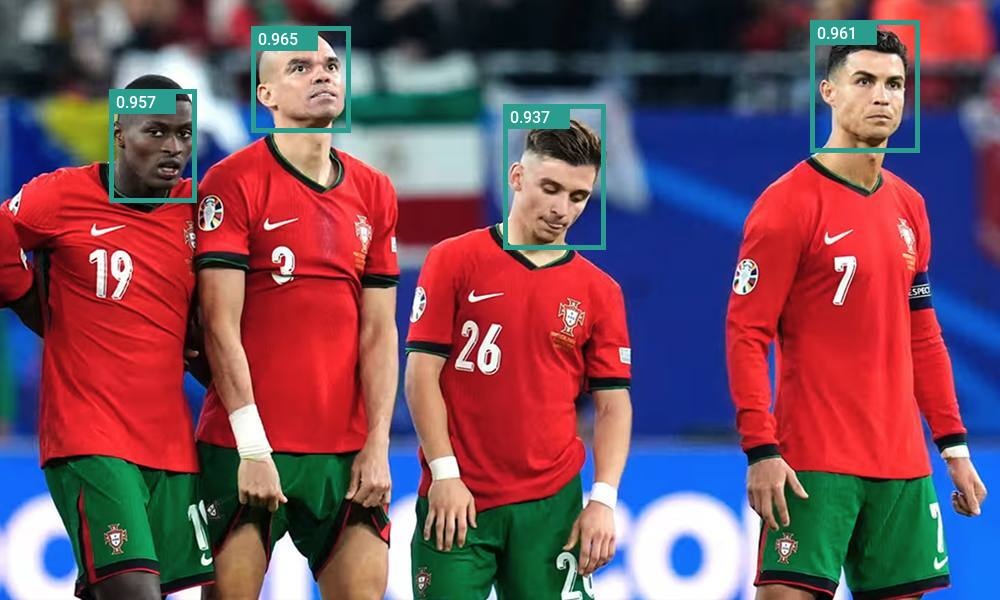
\includegraphics[width=.95\linewidth]{paper_assets/xface_multi_face_rknn_result.jpg}
  \centering\scriptsize RKNN INT8 trên Luckfox RV1106 phát hiện đủ 4/4 khuôn mặt.
  \column{0.41\textwidth}
  \footnotesize
  \begin{block}{Kết luận}
  \begin{itemize}
    \item Hoàn thiện quy trình training $\rightarrow$ YOLOv5s $\rightarrow$ RKNN INT8.
    \item Accuracy được duy trì tốt trên RV1106; ứng dụng hoạt động hoàn toàn trong mạng nội bộ.
  \end{itemize}
  \end{block}
  \begin{block}{Hướng phát triển}
  \begin{itemize}
    \item Bổ sung landmark khuôn mặt và mở rộng dữ liệu góc nghiêng, ánh sáng.
    \item Lưu lịch sử điểm danh lâu dài.
  \end{itemize}
  \end{block}
\end{columns}
\end{frame}

\end{document}
